\chapter{Tecnologias}
\label{tecnologias}
Este capítulo tem como foco explicar cada uma das tecnologias propostas neste texto para resolver o problema de escalabilidade. 

Primeiramente na seção \ref{sec: MEAN} explicaremos o conceito da sigla MEAN, e as subseções seguintes detalharão cada uma das tecnologias, sendo que na subseção \ref{subsec: MongoDB} será explicado o MongoDB, na subseção \ref{subsec: Express.js} falaremos sobre o Express.js, na subseção \ref{subsec: AngularJS} abordaremos sobre o AngulaJS e na última subseção \ref{subsec: Node.js} nos focaremos no Node.js. No final deste capítulo na seção \ref{subsec: Socket.io} explicaremos um pouco sobre o Socket.io.

\section{MEAN Stack}
\label{sec: MEAN}
O nome MEAN é uma sigla que representa o conjunto de 4 ferramentas:
o banco de dados NoSQL \textbf{M}ongoDB\footnote{http://www.mongodb.org/}, o framework back-end \textbf{E}xpress\footnote{http://expressjs.com/} , o framework front-end \textbf{A}ngularJS\footnote{https://angularjs.org/}, e o servidor \textbf{N}odeJS\footnote{http://nodejs.org/}. Nos subtópicos abaixo serão abordadas as principais características de cada uma dessas ferramentas.

\subsection{MongoDB}
\label{subsec: MongoDB}
O MongoDB é um banco de dados de código aberto do tipo NoSQL. Foi implementado na linguagem  C++ e é orientado a documentos. O formato dos documentos utilizados pelo MongoDB é o JSON\footnote{\textit{JavaScript Object Notation}, é um formato de texto baseado no conceito de chave-valor, que serve para troca de informações/dados entre sistemas.}/BSON\footnote{Internamente este formato é convertido para BSON, que é um arquivo JSON no formato binário, que foi criado para tornar mais eficiente a busca e o espaço de armazenamento.}, utiliza-se este formato pela facilidade na integração de dados em certos tipos de aplicações. O nome Mongo vem da expressão da língua inglesa ``humongous'',  que significa ``monstruoso'' ou ``gigantesco''. 

Algumas razões por optarem pelo Mongo para funcionar junto com ferramentas Javascript, é que além de tratar objetos JSON, e de estar sendo bem aceito pela comunidade\cite{dbEng}, ele possui um bom desempenho com grande volume de dados \cite{compBds}, e com ele também é possível se executar códigos em Javascript  para as consultas, além de possuir uma grande integração\footnote{Através do próprios drives, e com a utilização da api Mongoose.} com Node.js.   

A figura \ref{fig:Gráfico comparando as terminologias do SQL e do MongoDB} \cite{MongoDbSQL} apresenta várias terminologias e conceitos padrões do SQL e as terminologias e conceitos correspondentes que o MongoDB utiliza.

\begin{figure}[!ht]
\centering
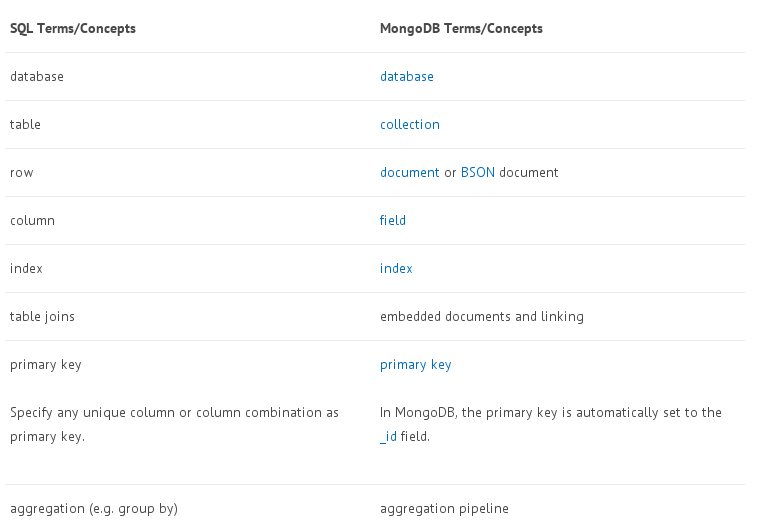
\includegraphics[scale=0.7]{images/comp_mongo_sql.png}
\caption{Gráfico comparando as terminologias do SQL e do MongoDB.}
\label{fig:Gráfico comparando as terminologias do SQL e do MongoDB}
\end{figure}

\begin{description}
\item[Escalabilidade através do Sharding] \hfill \\ 
 O termo \textit{Sharding} é uma técnica de escalabilidade horizontal em que os dados de uma base de dados são divididos em muitos \textit{Shards}, os quais podem ser distribuídos entre várias máquinas \cite{AnalysisNoSQL}.

O MongoDB tem suporte a uma técnica conhecida como \textit{Autosharding}, que ``permite a construção de um \textit{cluster} de banco de dados escalável horizontalmente projetado para incorporar novas máquinas de forma dinâmica'' \cite{BdNoSQLxSGBDs}.

O \textit{cluster} é formado de três componentes: Blocos de servidores chamados \textit{Shards}, que são reponsáveis pelo armazenamento dos dados, os servidores de configuração chamados de \textit{mongod}, que contém os meta-dados e as informações de rotas, e os serviço de rotas chamados \textit{mongos}, que é responsável ``pelo roteamento das operações ao destino apropriado''\cite{BdNoSQLxSGBDs}.

A figura \ref{fig: Topologia do Sharding} \cite{MongoPy} abaixo mostra como os componentes que constituem o \textit{cluster} do MongoDB interagem para prover uma escalabilidade horizontal.  
\begin{figure}[!ht]
\centering
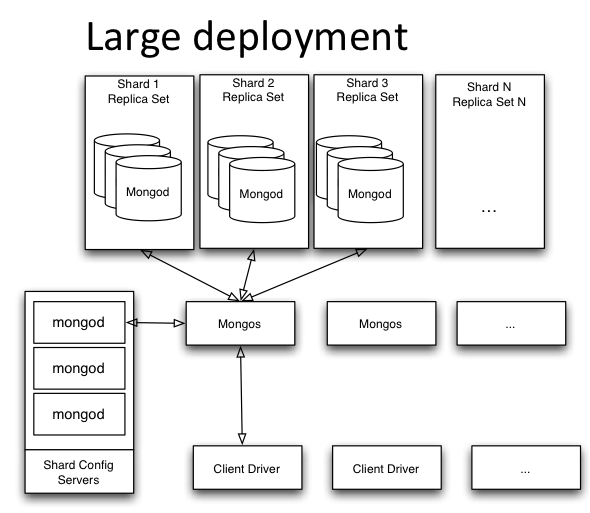
\includegraphics[scale=0.7]{images/1sharding_topology.png}
\caption{Topologia do Sharding.}
\label{fig: Topologia do Sharding}
\end{figure}

\item[Armazenamento] \hfill \\
O MongoDB utiliza arquivos mapeados em memória, ``que mapeia diretamente um arquivo armazenado em disco para um array de bytes em memória virtual, não memória física RAM, onde a lógica de acesso aos dados é implementado usando aritmética de ponteiro. O uso de arquivos mapeados em memória é eficiente para melhorar o desempenho''\cite{AnaliseNosql}.

Uma das características do MongoDB é a de ter Consistência eventual (\textit{Eventual consistency}), que significa que  existe um momento devido para o sistema tornar-se consistente. \cite{BaseAcid}

O gerenciador de memória virtual do sistema operacional é responsável por decidir quais partes da base de dados vão para o disco e quais ficam em memória. Este mecanismo faz com que o MongoDB não tenha controle sobre quando os dados são escritos no disco\cite{AnalysisNoSQL}.

\end{description}


\subsection{Express.js}
\label{subsec: Express.js}
O Express é um \textit{framework} que visa facilitar o desenvolvimento de aplicações Web com o Node.js. O Express.js permite criar servidores web e receber requisições HTTP de maneira simples, além de também permitir a criação de um conjunto de diretórios com uma estrutura padrão e organizar as rotas dos arquivos para as views da aplicação. Geralmente os projetos que utilizam-se do Express também aderem há algum framework de \textit{templates} como Jade ou EJS.

\subsection{AngularJS}
\label{subsec: AngularJS}
AngularJS é um framework javascript \textit{client-side} que segue o modelo MVC\footnote{MVC (\textit{Model-view-controller}, que em português é Modelo-Visão-Controlador) é uma forma de estrutura seu projeto/aplicação de forma que a interface de interação (\textit{views}) esteja separada do controle da informação em si (\textit{models}), separação essa que é intermediada por uma outra camada controladora (\textit{controlers}).} e é mantido pela Google.

Existem muitos outros frameworks além do AngularJS, porém ao meio de tanta competitividade ele tem se destacado, o gráfico abaixo é um bom argumento para mostrar a popularidade do Angular.

A figura \ref{fig:Gráfico Comparando Frameworks Javascript} foi retirada do site ``Info Q \cite{fwJs}'', onde realizam uma enquete para saber qual framework é mais utilizado pelos desenvolvedores, a enquete é realizada como um drag and drop, no caso o usuário que está votando terá que arrastar o nome da aplicação para o gráfico e posicionar ele entre os dois eixos de acordo com sua opinião.

A linha vertical, \textit{``Value Proposition''}, representa a importância da aplicação para o usuário que está votando, a linha horizontal, \textit{``Adoption Readiness''} representa o quanto o usuário usa a aplicação na vida real. 

 No resultado final desta enquete, ou seja, a média dos votos, temos os pequenos círculos que representam cada framework e o tamanho deste círculo representa a quantidade de votos, ou seja se o círculo é grande logo a aplicação recebeu muitos votos.

\begin{figure}[!ht]
\centering
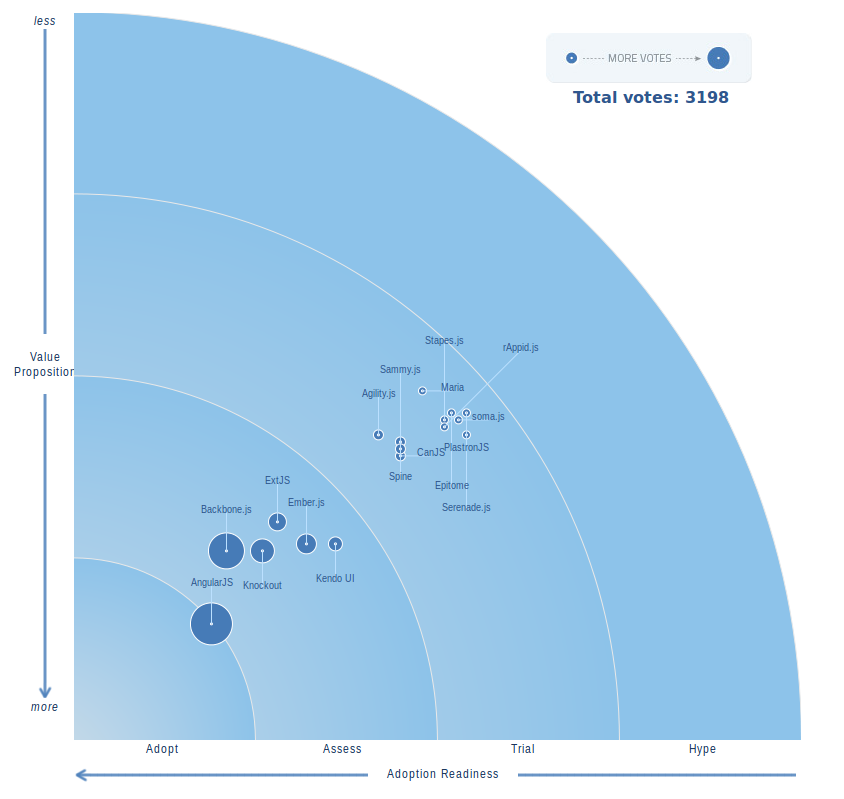
\includegraphics[scale=0.5]{images/angularjs_framework_comparison.png}
\caption{Gráfico comparando frameworks Javascript.}
\label{fig:Gráfico Comparando Frameworks Javascript}
\end{figure}

\newpage

Algumas características que se destacam no AngularJS são:
\begin{description}
\item[SPA - Single Page Application] \hfill \\ 
O conceito de Single Page Application é  quando cada parte de página é carregada de forma independente, ou seja, quando uma página é carregada, todas as demais atualizações são feitas através de requisições AJAX\footnote{AJAX é uma metodologia que utiliza tecnologias como XML e Javascript para fazer requisições assíncronas ao servidor e com as informações retornadas modificar uma página carregada através do DOM, sem a necessidade de recarregar todo seu conteúdo.} e renderizações parciais na página.

    Através destas renderizações parciais temos um aumento de performance devido a diminuição da quantidade de dados que precisam ser trafegadas entre o cliente e o servidor.

\item[Two-Way Data Biding] \hfill \\
É recurso para facilitar o desenvolvimento do sistema enquanto o AngularJS manipula e cuida de atualizar as informações da pagina. Através do uso de alguns controles na pagina em HTML o AngularJS consegue identificar e mapear os atributos a serem atualizados.

\item[Injeção de dependências] \hfill \\
A injeção de dependências consiste basicamente  em fornecer recursos extras necessários na aplicação de forma transparente ao usuário, de modo que o desenvolvedor somente deverá solicitar um recurso, que será injetado pelo \textit{framework} e ficará disponível para uso.
\end{description}

\subsection{Node.js}
\label{subsec: Node.js}
\nocite{poeNode}
\nocite{MongoNode}
O Node.js é uma plataforma de desenvolvimento web que funciona com a linguagem Javascript no lado do servidor, para criação de aplicações e páginas web de alta escalabilidade, sendo que foi concebida por  Ryan Dahl em 2009 \nocite{appRealTime}, e desde então vem ganhando muita popularidade entre os desenvolvedores web, e sendo utilizado por grandes empresas e instituições tais como LinkedIn, Microsoft, GitHub, MySpace, entre outras\cite{compNode}.

A escolha da linguagem Javascript foi devido a enorme quantidade de bibliotecas para I/O que a linguagem possui, permitindo assim criar as funções assíncronas para a plataforma.

A arquitetura do Node.js é composta em sua maior parte por componentes  desenvolvidos em C e em Javascript \nocite{nodeInAction}. Os principais componentes da parte escrita em C são: a \textit{V8 Javascript Engine}\footnote{É máquina virtual para Javascript do Google utilizada no navegador Chrome, que ``compila e executa código fonte JavaScript, lida com a alocação de memória para objetos e limpa-os quando não são mais necessários''\cite{v8Eng}.}, o \textit{Node Bindings}\footnote{São códigos executáveis que fazem com que o V8 e a biblioteca em javascript padrão do node sejam capazes de se comunicar.}, a  \textit{Thread Pool}\footnote{``É uma coleção de threads disponíveis para realizar tarefas''\cite{ThreadPool}}, e o \textit{Event Loop}. Para a parte responsável pelo Javascript, foi criada uma biblioteca chamada \textit{Node Standard Library}, para permitir que o Node.js interprete códigos em Javascript.

Abaixo segue a figura \ref{fig:Arquitetura do Node.js} \cite{nodeMeet} que concede um modelo visual desta arquitetura, com o intuito de facilitar o entendimento da relação entre os componentes citados do Node.js.

\begin{figure}[htb]
\centering
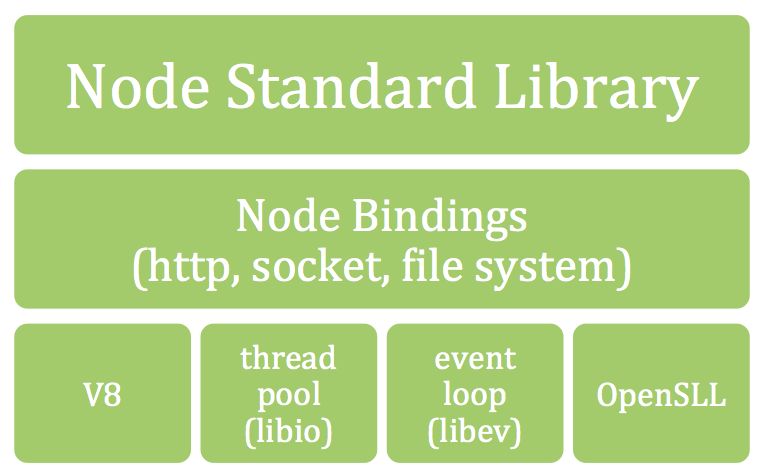
\includegraphics[scale=0.4]{images/node_platform.png}
\caption{Arquitetura do Node.js.}
\label{fig:Arquitetura do Node.js}
\end{figure}
    
    O Node.js foi criado de forma que suas funcionalidades pudessem ser estendidas através de módulos, para implementar diversos componentes middleware que facilitem o desenvolvimento de aplicações web. Estes módulos são geralmente instalados através de um gerenciador de pacotes conhecido como npm, que significa \textit{Node Package Manager}, e serve para facilitar diversos aspectos relacionados a aplicação como a compilação, a instalação e a atualização, e também funciona como um gerenciador de dependências.

\begin{description}
\item[I/O não bloqueante e orientado a eventos] \hfill \\
Quando necessitamos acessar\footnote{Seja para leitura, escrita, atualização ou remoção.} os dados de uma aplicação, estes dados podem estar em vários locais, tais como na memória (L1, L2, RAM), no disco ou na rede, e cada local contem uma latência de I/O diferente, no caso para memória quando necessitamos acessar a L1 gastamos aproximadamente  3 ciclos, passando para 14 ciclos na L2 e para 250 ciclos na RAM, já para o disco e para a rede a quantidade de ciclos necessários tem um aumento significativo, sendo aproximadamente 41 e 250 milhões de ciclos, respectivamente, ou seja, quando utilizamos a memória podemos considerar que será um acesso rápido, também conhecido como não bloqueante, e já para o disco e a rede consideramos que será um acesso lento, também conhecido como bloqueante.

A figura \ref{fig:Event Loop do Node.js} \cite{nodeMeet} demonstra como é o funcionamento do \textit{Event Loop} no Node.js, que tem como entrada uma fila (\textit{queue}) de requisições, e no caso de ser recebido uma requisição bloqueante, esta requisição é passada para uma \textit{Thread Pool}, que irá tratar o evento, caso contrário o evento é tratado no próprio \textit{Event Loop}.

\begin{figure}[ht]
\centering
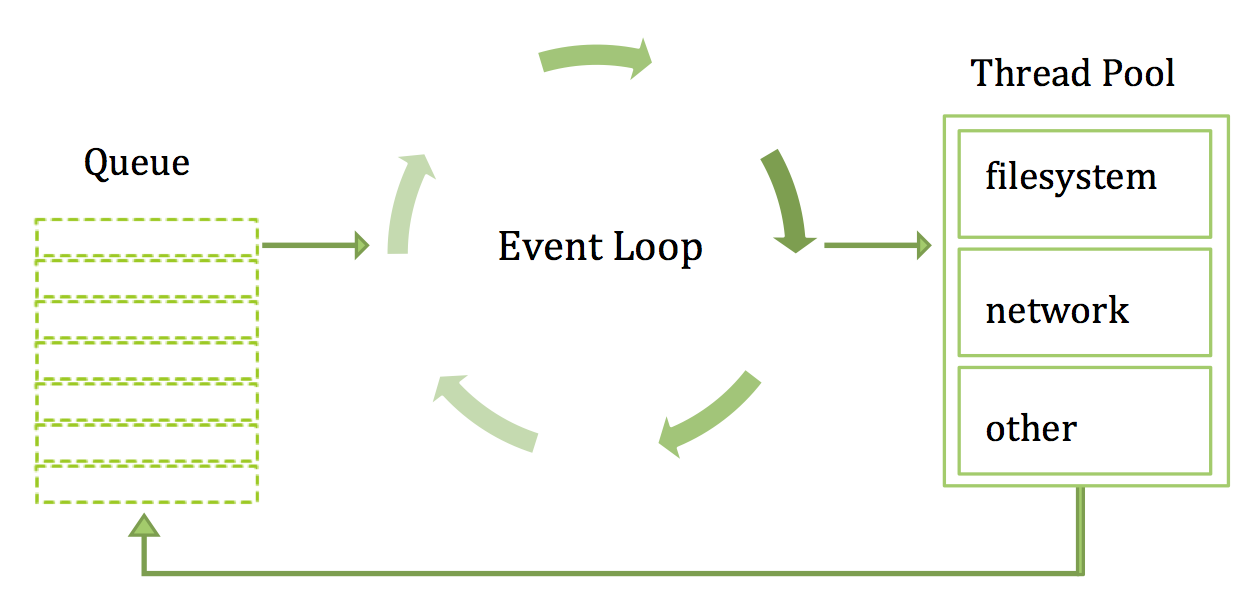
\includegraphics[scale=0.3]{images/node_event_loop.png}
\caption{Event Loop do Node.js.}
\label{fig:Event Loop do Node.js}
\end{figure}

O Node.js foi desenvolvido com base no conceito de ``I/O não bloqueante''\nocite{nodeRight}  (também conhecido por I/O assíncrono), e isto foi feito através da utilização e adaptação de uma construção  de programação conhecida como \textit{Event Loop}, que foi explicado na seção \ref{sec:Programação orientada a eventos} do capítulo \ref{cha: Conceituação e Idéia Geral}.

A execução do Node.js geralmente funciona através de uma única \textit{thread}, e quando existe a necessidade de I/O bloqueante uma \textit{Thread Pool} fica responsável por lidar com este tipo de I/O.  

Um exemplo do funcionamento do \textit{Event Loop} do Node.js é quando se recebe uma requisição de um evento não bloqueante, sendo que este evento será tratado diretamente pela \textit{thread} principal, e outra situação é quando se recebe uma requisição bloqueante, como por exemplo uma leitura de disco, esta requisição então é enviada para a \textit{Thread Pool} do Node.js, que irá utilizar uma \textit{thread} para tratá-la, e quando terminar, a \textit{thread} responsável pelo processamento bloqueante envia uma mensagem para a \textit{thread} principal que então executa a função de \textit{callback}\footnote{''é um mecanismo de controle de fluxo que visa beneficiar processos assíncronos.''\cite{StackOCallbk}} respectiva a requisição.
    
\end{description}

\section{Socket.IO}
\label{subsec: Socket.io}
O Socket.io é uma API em Javascript que permite que a comunicação entre o servidor e o cliente ocorra sem dificuldades e em tempo real. Ele abstrai e utiliza o protocolo \textit{WebSocket}\footnote{É um protocolo orientado a eventos que permite abrir uma sessão de comunicação interativa entre o navegador do cliente e o sevidor, sendo possível enviar mensagens para um servidor e receber respostas sem ter que consultar o servidor para uma resposta.},  e também possui outras alternativos caso seja um ambiente que não suporte \textit{WebSocket}.